% Springer Nature journal article template, version 3.1 (December 2024).
% LRE's journal-specific requirements supplement the generic template.
\documentclass[pdflatex,sn-basic]{sn-jnl}

\usepackage[utf8]{inputenc}
\usepackage{graphicx}
\usepackage{amsmath,amssymb}
\usepackage{booktabs}
\usepackage{longtable}
\usepackage{tabularx}
\usepackage{array}
\usepackage{xcolor}
% Keep the PDF outline within the section/subsection hierarchy; the official
% class's \bmhead command uses subparagraph level 5 for declarations.
\hypersetup{bookmarksdepth=2}

\newcommand{\promptfinal}{\texttt{full\_prompt\_final}}
\newcommand{\metafree}{\texttt{metadata\_free\_prompt\_final}}
\newcommand{\targetfinal}{\texttt{target\_final\_subtoken}}
\newcommand{\targetmean}{\texttt{target\_mean\_span}}
\newcommand{\bfana}{\texttt{bf16-analysis-20260826-v2}}
\newcommand{\repo}{\texttt{research-stack}}

\title{Lexical Split Design and Representation-Interface Validity in
Decoder-Only Morphology Probing: An Arabic Evaluation Study}

\author*[1]{\fnm{Mohammed} \sur{Al-Thobaiti}}\email{mthobaiti@outlook.com}
\affil*[1]{\orgname{Independent researcher},
\orgaddress{\city{Jeddah}, \country{Saudi Arabia}}}

\begin{document}

\abstract{%
Diagnostic classifiers are often evaluated with random instance splits even
when lexical identity is correlated with the target label. This paper treats
split design and representation-interface design as measurement choices in
decoder-only morphology probing. Using Arabic morphology as a testbed, we
evaluate eleven pinned Hugging Face models with BF16 hidden-state captures,
three morphology tasks, three split conditions, and four representation
interfaces. The evaluation uses deterministic nested five-fold procedures,
development-only layer selection, fixed Ridge classification, shuffled-label
controls, validated token alignment, and checksummed artifacts. Across the 132 model--task--
interface comparisons, random-split macro-F1 is higher than both lemma-heldout
and root-heldout macro-F1. The random-minus-lemma differences range from
0.0127 to 0.2863 (mean 0.1059), and random-minus-root differences range from
0.0255 to 0.2796 (mean 0.1179). Effects vary by model, task, and interface;
the range rules out a single summary penalty. A full-metadata prompt-final
state compares position together with information availability: the prompt
explicitly supplies lemma, root, and pattern. A
metadata-free prompt-final condition and target-span pooling expose these
confounds while holding the dataset and probe fixed. The results support
claims about linear recoverability under named prompts, splits, token spans,
and estimators; questions about causal model use, linguistic competence, and
behavior in other settings require separate evidence. Planned
post-extraction analyses can use archived representations and derived artifacts
alone.
}

\keywords{Probing, lexical leakage, split design, Arabic morphology,
decoder-only models, reproducibility}

\maketitle

\section{Introduction}

Diagnostic classifiers are useful because they make a representation's
accessibility testable with a comparatively simple estimator. A probe that
predicts a linguistic label from a hidden state requires an explicit account
of its measurement conditions. The result can depend on
which examples are placed together, which information the prompt supplies,
where the hidden state is extracted, how subword tokens are aligned to the
stimulus, and how imbalanced labels are scored. Work on probing has therefore
emphasized control tasks, selectivity, and careful interpretation
\citep{hewitt-liang-2019,hewitt-manning-2019,tenney-etal-2019-iclr,
ravichander-etal-2021}.

This paper studies one particularly consequential evaluation choice: whether
the test set contains lexical identities or lexical families that also occur
in training. Under a random instance split, repeated lemmas, roots, or related
surface forms can appear on both sides of the partition. If those identities
are correlated with morphology, a probe can obtain a high score while being
tested mainly on interpolation within a familiar lexical inventory. A split
that holds out lemma or root groups asks a different question: how much of the
label remains linearly recoverable when the grouping identity is absent from
training? Random splitting serves as a legitimate optimistic reference for
instance-level interpolation; its interpretation remains distinct from lexical
generalization across heldout identities. The distinction follows the broader
warning that standard and random splits can be misaligned with the intended
generalization claim \citep{gorman-bedrick-2019,sogaard-etal-2021}.

Arabic provides a useful testbed because lexical, templatic, and inflectional
structure interact. Lemmas and roots define meaningful grouping variables, yet
holding them out leaves semantic, orthographic, and morphological relations
available across partitions. The setting therefore supports a direct
evaluation of lexical split sensitivity while leaving the broader open-set
language question unresolved. Arabic resources also make the tokenization
problem concrete: a morphological word may span multiple subword units, and
different tokenizers segment the same stimulus in different ways
\citep{taji-etal-2017,sennrich-etal-2016,
bostrom-durrett-2020}.

Split design is only one interface choice. A decoder-only prompt-final state
has processed the target, the instruction, and any fields that follow the
target. In the full-metadata condition used here, lemma, root, and pattern are
explicitly present. A target-final state is extracted from a causal prefix
ending at the final target-overlapping token, excluding those later fields. A
comparison between these states therefore changes
both position and available information. We add a metadata-free prompt-final
condition to isolate part of that confound and retain the complete target span
so that final-subtoken and mean-span representations can be derived locally.

The central contribution is a methodological evaluation of lexical split
validity and representation-interface validity in decoder-only morphology
probing, with Arabic morphology as the testbed. The study uses the completed
BF16 matrix, with the historical Q8 run serving as robustness context. Its
contribution is an audited account of the decisions that determine what a
probe score means, together with archived representations that make later
analyses independent of renewed model inference.

We ask four questions:

\begin{enumerate}
    \item \textbf{Split validity:} How much do random-instance macro-F1
    estimates differ from lemma-heldout and root-heldout estimates under the
    same task, model, and representation interface?
    \item \textbf{Interface validity:} How do full-metadata prompt-final,
    metadata-free prompt-final, final target-subtoken, and mean target-span
    interfaces differ when the information available at each site is stated
    explicitly?
    \item \textbf{Model heterogeneity:} Are split effects stable enough to
    report as one penalty, or do they vary across model families, sizes, and
    morphology tasks?
    \item \textbf{Reproducibility:} Can complete, validated BF16 captures
    support the planned local analyses using archived captures alone?
\end{enumerate}

The principal findings are descriptive. Random-split macro-F1 exceeds both
grouped heldout conditions in every row of the generated 132-row comparison
table, but the differences range substantially. The full-metadata prompt-final
interface is often the strongest absolute condition in aggregate, while the
metadata-free and target interfaces retain substantial signal in many cells.
The exact ordering changes across tasks and models. These patterns support a
methodological recommendation: probing reports should state the lexical unit
held out, the information available at the extraction site, the pooling rule,
and the estimator-selection boundary. Linear probe performance should be
interpreted as recoverability under those conditions, with causal use and
linguistic competence treated as separate questions.

\section{Background and Related Work}

\subsection{Probing and diagnostic classifiers}

Probing studies use a classifier or structured estimator to ask whether a
property is accessible from a representation. Structural probes, layer-wise
diagnostics, and contextual analyses have made this approach a productive way
to inspect learned representations \citep{hewitt-manning-2019,
tenney-das-pavlick-2019,tenney-etal-2019-iclr}. The appeal of a linear probe is
also its limitation: a successful classifier establishes a property of the
representation--estimator pair. Its relationship to the model's generation
mechanism requires separate evidence. A linear classifier can exploit distributional
regularities that are unrelated to the model's causal computation for a task.

Probe capacity and controls matter. A high-capacity probe can recover
information that is present in a distributed or incidental form, and a low
score can reflect a mismatch between the estimator and the representation,
leaving property recoverability unresolved. Control tasks and shuffled labels are
therefore useful sanity checks, while selectivity and task relevance require
separate reasoning \citep{hewitt-liang-2019,ravichander-etal-2021}. We use a
fixed standardized Ridge classifier as a deliberately limited, reproducible
measurement. Our claims concern linear recoverability under that estimator;
other probe classes constitute separate measurements.

\subsection{Lexical memorization and split design}

The random split convention is attractive because it is simple and often
produces balanced partitions. It can nevertheless give an optimistic estimate
when examples are clustered by a lexical or document identity. The same
split-design issue arises across empirical tasks: correlated observations can
be distributed across training and test while the intended generalization unit is
obscured \citep{gorman-bedrick-2019,sogaard-etal-2021}. In a
morphology resource, lemma and root are natural grouping candidates because
they capture recurrent lexical structure. The choice is substantive: a
lemma-heldout score asks about transfer across lemmas, while a root-heldout
score asks about transfer across a broader and linguistically different group.

Our design treats random performance as a reference condition and measures its
gap from two grouped conditions. The gap is evidence that evaluation depends on
lexical composition; it measures split sensitivity, while the source of that
sensitivity remains distributed across several possible leakage paths. Related
surface forms, morphology patterns, meanings, source-document regularities,
and tokenizer fragments may cross a lemma or root boundary.

\subsection{Morphology probing and Arabic resources}

Morphological labels are attractive probing targets because they are structured
and can be attached to individual word forms. They are also heterogeneous:
part of speech, gender, and number differ in class cardinality, imbalance, and
the extent to which their cues are tied to lexical identity. Accuracy can hide
poor minority-class behavior, especially for three-way number classification;
macro-F1 is consequently reported alongside accuracy and the training-only
majority baseline.

Arabic adds both linguistic and resource-specific issues. Universal
Dependencies Arabic-PADT provides a documented dependency-treebank resource
for Arabic \citep{taji-etal-2017}; CAMeL Tools provides open-source Arabic
processing infrastructure \citep{obeid-etal-2020}. Morphological analyzers
can supply rich features but also introduce analyzer-specific conventions,
ambiguity decisions, and normalization choices. This paper treats the
resulting annotations as a constructed evaluation resource with recorded field
lineage and bounded coverage of Arabic morphology. Recent Arabic analyzers
illustrate both the value and the
continuing engineering requirements of such resources
\citep{khairallah-etal-2024}.

\subsection{Decoder-only extraction, tokenization, and pooling}

Decoder-only models expose a sequence of causal hidden states along the
prompt, and word representations vary with the extraction location. The state at
the end of a prompt can summarize fields that follow the target; the target
state excludes those later fields. Subword tokenization further means that a target word may occupy one,
two, or more tokenizer pieces. Subword units are useful for efficient language
modeling \citep{sennrich-etal-2016}, while their boundaries can diverge from
morphological boundaries, and tokenizer choices affect which state is called
the ``word'' state \citep{bostrom-durrett-2020}. We therefore save every
target-overlapping token state and derive final-subtoken and mean-span pooling
after extraction. The pooling comparison tests robustness of the measurement
interface and leaves linguistic canonicality as an open question.

\subsection{Evaluation and reproducibility methodology}

Reproducibility in representation probing has two layers. The statistical
pipeline must prevent test information from selecting layers, preprocessing,
or hyperparameters. The extraction pipeline must make model identity,
tokenizer identity, prompts, target spans, tensor semantics, and file
integrity inspectable. We address both layers with deterministic manifests,
structural alignment checks, content hashes, and independently validated
per-model bundles. This is especially important when model inference is
performed on ephemeral GPU instances and subsequent scientific analysis is
intended to run locally.

\section{Evaluation Resource}

\subsection{Source resource and release identity}

The authoritative input is a 4,701-row normalized JSONL artifact derived from
the official Universal Dependencies Arabic-PADT repository:
\url{https://github.com/UniversalDependencies/UD_Arabic-PADT}. The local
record identifies the earliest matching official release as r2.17 and retains
the archived commit and the SHA-256 of the training file. The original source
copy lacks Git metadata, and the same training-file content is byte-identical
in official r2.17 and r2.18. The repository therefore records the release
ambiguity and leaves the historical local label unresolved. The upstream license is CC BY-NC-SA 3.0; the archived license
file is retained with the source material. No acquisition date was recorded.

Only the PADT training file enters the construction pipeline. The archived
development and test files are retained for provenance only. ``Train,''
``development,'' and ``test'' in the probing evaluation refer to newly
constructed folds, distinct from the original UD file partitions.

\subsection{Construction and field lineage}

The resource construction is deterministic and has two conceptually distinct
stages. First, the pipeline reads eligible PADT tokens in source order,
disambiguates complete sentences with CAMeL Tools 1.6.0 and the
\texttt{calima-msa-r13} MLE model, takes the top analysis, and stops after
5,000 retained candidates. The construction consumed 330 sentence units and
11,437 source tokens before writing those candidates. Second, it normalizes
the analyzer output, requires lemma, root, abstract pattern, and concrete
pattern, removes ambiguous records, and retains normalized POS values NOUN,
VERB, and ADJ. The strict filter removes 299 records and leaves 4,701.

The field lineage is explicit:

\begin{itemize}
    \item \texttt{surface} is the analyzer/PADT surface form and
    \texttt{surface\_dediac} is the normalized form produced by the recorded
    Arabic diacritic and formatting-mark removal routine.
    \item \texttt{lemma}, \texttt{root}, \texttt{abstract\_pattern}, and
    \texttt{concrete\_pattern} are analyzer-derived fields after the recorded
    normalization and ambiguity filtering.
    \item \texttt{pos}, \texttt{gender}, and \texttt{number} are task labels
    selected from the normalized analyzer fields. POS has classes NOUN, VERB,
    and ADJ; gender has fem and masc; number has sg, pl, and du.
    \item \texttt{id} is an immutable stimulus identifier. Source identity,
    source split metadata, and the construction provenance string are retained
    as metadata for grouping and audit, separate from model inputs.
\end{itemize}

The frozen JSONL contains 1,519 unique lemmas, 707 unique roots, and 2,331
unique surface forms. POS counts are 2,957 NOUN, 910 ADJ, and 834 VERB.
Gender is available for 4,699 rows: 2,942 masculine and 1,757 feminine,
with two missing values. Number is available for 4,699 rows: 3,954 singular,
700 plural, and 45 historical dual labels stored as \texttt{def}, with two
missing values. The historical spelling is preserved byte-for-byte. At task
load, only the number field is canonicalized from \texttt{def} to the semantic
label \texttt{du}; the dataset artifact remains byte-for-byte unchanged.

The cross-tabulation of the three primary labels after this task-specific
canonicalization is shown in Table~\ref{tab:pos-gender-number}. It covers the
4,699 rows with all three labels and is included to make the class composition
visible; it introduces no new evaluation target.

\begin{table}[t]
\centering
\caption{Counts by POS, gender, and number for rows with all three primary
labels. The 45 stored \texttt{def} values are counted as semantic \texttt{du}
for this descriptive table.}
\label{tab:pos-gender-number}
\scriptsize
\begin{tabular}{lrrrrrr}
\toprule
 & \multicolumn{3}{c}{Masc.} & \multicolumn{3}{c}{Fem.} \\
POS & sg & pl & du & sg & pl & du \\
\midrule
NOUN & 1580 & 388 & 25 & 712 & 243 & 8 \\
ADJ  & 415 & 17 & 1 & 471 & 1 & 4 \\
VERB & 464 & 48 & 4 & 312 & 3 & 3 \\
\bottomrule
\end{tabular}
\end{table}

The field definitions describe this constructed resource with its analyzer
ambiguity conventions. The probe unit is an eligible PADT token. No new clitic
segmentation is introduced by the probing adapter. Patterns, roots, and lemmas
are retained for grouping, metadata, and audit purposes; high-cardinality label
prediction falls outside the primary task scope.

\subsection{Original construction split and probing folds}

For historical dataset construction, the vendored pipeline recorded a
root-heldout split with seed 17 and nominal 0.70/0.15/0.15 proportions: 3,291
training, 705 development, and 705 test records. This construction split is
distinct from the evaluation split used for the reported five-fold results.
The latter is generated independently at task load from the frozen example order, as
specified in Section~\ref{sec:methodology}.

\subsection{Released and archived artifacts}

The resource package includes the normalized stimulus file, source and
transformation provenance, source-content hashes, the vendored construction
pipeline, task-specific fold manifests, prompt specifications, BF16 model
manifest, representation-bundle manifests, derived representations, result
tables, prediction records for the primary models, validation reports, and
checksums. Large hidden-state arrays are recorded as external artifacts in the
BF16 freeze; their hashes and bundle identities are preserved, while any public
redistribution must respect the relevant model licenses. The scientific
evidence package contains representation artifacts and metadata; model weights
remain external.

\section{Evaluation Methodology}\label{sec:methodology}

\subsection{Evaluation questions and split conditions}

Each task is evaluated under three split conditions. The random condition
uses nested five-fold stratified partitioning with seed 42. It is the
optimistic reference for ordinary instance-level interpolation. The
lemma-heldout condition uses nested five-fold GroupKFold with lemma as the
grouping key. The root-heldout condition uses the same procedure with root as
the grouping key. For each outer fold, the test partition is the selected
outer fold and the development partition is fold zero of a second partition
over the outer-training data. The remaining data are training data.

The grouping conditions answer different questions. Lemma holdout keeps each
lemma identity within a single partition; root holdout applies the same rule
to each root identity. Direct set-intersection audits verify zero overlap of
the applicable grouping key across training, development, and test in every
recorded fold. These controls reduce direct lexical recurrence while leaving
semantic, orthographic, morphological, and source-document correlations
available across partitions. Random splitting remains the labeled reference
condition for instance-level interpolation.

Rows with a missing task label are removed before fold construction. Thus POS
uses all 4,701 records and gender and number use 4,699 records. The same
frozen example order and deterministic split generator are used across
representation interfaces for a given model and task.

\subsection{Probe, layer selection, and metrics}

The primary estimator is a pipeline consisting of a training-fitted
\texttt{StandardScaler} followed by \texttt{RidgeClassifier} with fixed
$\alpha=1.0$. For every outer fold and every layer, the scaler and probe are
fit on training examples only. Development accuracy selects the layer;
development macro-F1 is the first tie-breaker, followed by the lowest layer
index. The chosen layer is refit on training plus development examples and is
evaluated once on the outer test partition. Test labels and test metrics never
select a layer, regularization value, preprocessing operation, or model.

Accuracy and macro-F1 are both reported. Accuracy makes the majority control
transparent; macro-F1 weights classes equally and exposes the effect of poor
minority-class prediction. Across the five outer folds, the primary point
estimate is the arithmetic mean and the reported fold dispersion is the
population standard deviation across those five recorded test results. This
dispersion describes fold variation; the bootstrap intervals reported
elsewhere have a separate interpretation.

\subsection{Baselines and shuffled-label controls}

The majority baseline predicts the most frequent training label, with explicit
deterministic tie-breaking. It is computed separately for every task and
outer fold, never from the test labels. Shuffled-label controls are run for
the two primary models, all four interfaces, all three tasks, all three split
conditions, and all five folds. Labels are permuted independently within
training, development, and test before the same layer-selection and fitting
pipeline is run. The complete audit contains 360 shuffled cells. None exceeds
its corresponding train-only majority baseline. After the label relationship
is removed, the shuffled pipeline stays at the majority reference; probe
performance on the real labels remains evidence about estimator-accessible
information under the stated interface.

\subsection{Uncertainty and secondary diagnostics}

The full BF16 matrix is summarized primarily with five-fold means and fold
dispersion. A separate 10,000-replicate, gold-stratified prompt-cluster
bootstrap is preserved for the historical paired location comparisons of the
original primary analysis. That bootstrap uses exact rendered-prompt clusters,
applies the same multiplicities to both paired locations, and is conditional
on fixed probes, selected layers, partitions, and representations. It supplies
conditional paired intervals for the historical comparison; the complete
11-model BF16 matrix is summarized separately with fold-level results.
Fold standard deviations retain their separate role as fold-dispersion
summaries.

Fragmentation and error analysis are descriptive. Fragmentation is stratified
by target token count in bins 1, 2, and 3+. The error artifact records
per-class precision, recall, F1, support, confusion matrices, and recorded
gold-POS strata. CKA and RSA are retained as fixed-sample diagnostics over
600 examples for the two primary models at the final layer. They serve as
secondary diagnostics and remain outside layer selection, probe fitting, and
the primary claims.

\section{Prompt Conditions and Representation Interfaces}

\subsection{Frozen prompt templates}

The prompt version is \texttt{bf16-lre-prompts-v1}; chat templates are
disabled. The full-metadata template is:

\begin{verbatim}
Arabic morphology token probe.
Surface: {surface_dediac}
Token: {target}
Lemma: {lemma}
Root: {root}
Pattern: {abstract_pattern}
Predict the token morphology.
\end{verbatim}

The metadata-free template is:

\begin{verbatim}
Arabic morphology token probe.
Surface: {surface_dediac}
Token: {target}
Predict the token morphology.
\end{verbatim}

The rendered prompt, target text, character span, byte span, and prompt hash
are stored per example. The templates are frozen before model comparison and
remain unchanged during local analysis.

\subsection{Information availability at each interface}

The four interfaces are:

\begin{description}
    \item[Full-metadata prompt-final (\promptfinal)] The final hidden state
    of the complete full-metadata prompt. The model can attend to the target,
    instruction, surface, lemma, root, and pattern fields, including fields
    after the target. These fields provide metadata that can correlate with
    morphology. This interface is therefore a contextual prompt endpoint;
    comparisons with target states combine position and information
    availability.
    \item[Metadata-free prompt-final (\metafree)] The final hidden state of
    the metadata-free prompt. It retains the surface and target but removes
    lemma, root, and pattern fields. It partially isolates the contribution of
    information availability while retaining a prompt-final context and the
    same task labels.
    \item[Target-final subtoken (\targetfinal)] The state at the final
    tokenizer piece overlapping the target span. It is obtained from a causal
    prefix ending at that target-overlapping piece, excluding later prompt
    fields. It is derived from the complete target-span capture in the
    full-metadata bundle.
    \item[Target-mean span (\targetmean)] The arithmetic mean over all
    target-overlapping token states in the same causal prefix. It uses the
    complete target span and is derived locally after extraction using the
    existing forward pass.
\end{description}

The full-metadata prompt-final and target interfaces differ in both position
and information availability. The metadata-free condition narrows this gap
while retaining later instructional context; the target state remains
prefix-only. We therefore describe interface comparisons as construct-validity
analyses and report the conditions under which each location is evaluated.

\subsection{Why retain the complete span}

Saving the complete target span preserves later pooling choices. Each BF16
layer stores the concatenated hidden states for every token whose validated
offset overlaps the target byte span. The
local loader uses the recorded per-example token counts to derive the final
row and the mean of the complete span. This supports final-subtoken,
mean-span, and further target-span pooling analyses from the archived captures
alone.

\section{Models and Representation Extraction}

\subsection{Pinned model matrix}

The matrix contains eleven official Hugging Face repositories: three Qwen
models for a within-family size comparison, three Llama models for a
within-family size comparison, Gemma, Phi, and Mistral as cross-family
references, and Jais and ALLaM as Arabic-specialist references. The matrix is
intentionally heterogeneous: it mixes base and instruction-tuned checkpoints
and supports robustness across selected model families. Scale and training-data
effects remain outside this design.

Every model has a frozen model revision, tokenizer revision, and config
revision. These revisions are full commit SHAs in the machine-readable model
manifest and are reproduced in Appendix~\ref{app:models}. The requested
inference and saved tensor dtype is BF16. The manifest records native
checkpoint dtype separately: Jais is listed with a native FP32 checkpoint and
was loaded under the explicit BF16 extraction contract. The extraction contract
excludes FP16 or FP32 fallback, quantization, CPU offload, and revision
fallback.

\subsection{Extraction semantics}

The extractor uses the pinned Hugging Face revision and tokenizer, evaluation
mode, a single CUDA device, right padding, and no chat template. It captures
the embedding output and each transformer-block output before final model
normalization. Logits and final-normalized representations are separate
quantities outside these capture sites. Saved tensors are BF16. The capture
sites are embedding output, prompt-final state per layer, and all target-span
token states per layer; full sequence-by-full-layer activations are omitted.

At extraction time, the harness fails on any mismatch in access, revision
resolution, tokenizer identity, architecture, context length, or BF16
requirements relative to the manifest. The exact prompt and model metadata are stored with each
bundle. The completed analysis uses 22 validated model/condition bundles,
two prompt conditions per model, and four analysis units per model.

\subsection{Structural alignment and example identity}

The target is rendered from a designated field and its character and UTF-8
byte spans are recorded structurally. A fast tokenizer with offset mapping
must identify a contiguous complete overlap. The harness records token IDs,
sequence length, token pieces, target token indices, target token count, the
decoded target text, and the selected final overlapping token. It selects
representations only from this validated mapping; assumed position, row order,
\texttt{[-1]}, and unvalidated text reconstruction are excluded. Alignment and example identifiers must
remain in the same order, and any failure prevents successful completion.

Each of the 22 bundles contains 4,701 examples and 4,701 successful
alignments. The analysis audit therefore enters local probing only after
bundle checks, metadata order checks, tensor shape checks, and finite-value
checks pass. The complete analysis has 44/44 atomic model-by-interface units,
1,980 real result cells, and 360 shuffled result cells. All eleven models use
five outer folds for random, lemma-heldout, and root-heldout evaluation.

\subsection{Bundle and provenance schema}

The bundle schema is versioned as \texttt{bf16-hidden-state-bundle-v1}. Each
bundle records model and tokenizer identity, prompt condition and template,
dataset path and hash, example metadata, alignment records, representation
semantics, layer count, hidden size, device, requested and saved dtype, code
identity, command, and runtime metadata. Scientific files are covered by a
SHA-256 manifest. Completion is a separate atomic marker bound to the current
checksum manifest and a verified persistent destination. A partial bundle
remains ineligible for the successful marker.

This design matters scientifically because it separates model inference from
analysis. The local sufficiency audit confirms that the saved fields support
the split reconstruction, all planned pooling choices, layer curves, linear
probes, majority controls, shuffled controls, fragmentation bins, class/POS
error analysis, BF16/Q8 metric comparison, and CKA/RSA-compatible matrices.
The recorded post-capture contract is \texttt{weights\_required=false}.

\section{Results}

\subsection{Overview of the complete matrix}

The primary BF16 analysis contains 11 models, 4 representation interfaces, 3
tasks, and 3 split conditions, with 5 outer folds for every combination. It
therefore yields 396 summary rows (11 x 4 x 3 x 3) and 132 rows in the compact
random-minus-grouped macro-F1 comparison. The compact comparison defines
\[
\Delta_{\mathrm{lemma}} = F1_{\mathrm{random}} - F1_{\mathrm{lemma-heldout}},
\qquad
\Delta_{\mathrm{root}} = F1_{\mathrm{random}} - F1_{\mathrm{root-heldout}}.
\]

Every one of the 132 rows has positive values for both deltas. Across rows,
$\Delta_{\mathrm{lemma}}$ ranges from +0.0127 to +0.2863 with mean +0.1059,
and $\Delta_{\mathrm{root}}$ ranges from +0.0255 to +0.2796 with mean
+0.1179. These descriptive averages summarize five-fold means. The result
establishes a consistent direction in this resource and matrix, while the
range shows why a single universal ``leakage penalty'' would obscure the
observed variation.

\begin{table}[t]
\centering
\caption{Descriptive mean macro-F1 gaps by model. Each value averages the 12
task-by-interface rows for that model in the generated 132-row table. The
full model-by-task-by-interface table is archived as
\texttt{results/macro\_f1\_split\_deltas.csv}, Markdown, and TeX.}
\label{tab:model-deltas}
\small
\begin{tabular}{lrr}
\toprule
Model & Random--lemma & Random--root \\
\midrule
ALLaM-7B & +0.0637 & +0.0816 \\
Gemma-4-E2B & +0.1382 & +0.1518 \\
Jais-13B & +0.0711 & +0.0918 \\
Llama-3.1-8B & +0.0835 & +0.0895 \\
Llama-3.2-1B & +0.1881 & +0.2054 \\
Llama-3.2-3B & +0.1276 & +0.1279 \\
Mistral-7B & +0.0993 & +0.1117 \\
Phi-3-mini & +0.1036 & +0.1314 \\
Qwen2.5-1.5B & +0.1134 & +0.1188 \\
Qwen3-0.6B & +0.0977 & +0.1118 \\
Qwen3-8B & +0.0783 & +0.0750 \\
\bottomrule
\end{tabular}
\end{table}

Table~\ref{tab:model-deltas} shows the heterogeneity. The model-level mean
lemma gap ranges from +0.0637 for ALLaM-7B to +0.1881 for Llama-3.2-1B;
the root gap ranges from +0.0750 for Qwen3-8B to +0.2054 for Llama-3.2-1B.
These grouped means provide descriptive orientation. Model ordering remains
confounded by families, parameter counts, native training mixtures, instruction
status, tokenizers, and architecture.

\subsection{Effect of lexical split design}

The complete result is stronger than a two-model demonstration. For every
model, task, and interface, random-split macro-F1 is above the corresponding
lemma-heldout and root-heldout value. The positive difference is consistent
with random splitting allowing lexical identities or lexical families to be
shared across training and test. The grouped conditions measure a more
demanding form of transfer and leave open-set language generalization for
separate evaluation.

The gap varies across grouping keys. In the full table, root-heldout
gaps are larger on average than lemma-heldout gaps (+0.1179 versus +0.1059),
but the model-level ordering differs: Qwen3-8B has a slightly larger
lemma than root average, whereas most models have a larger root average. This
variation is a reason to report both controls and keep their grouping keys
visible.

\begin{figure}[t]
\centering
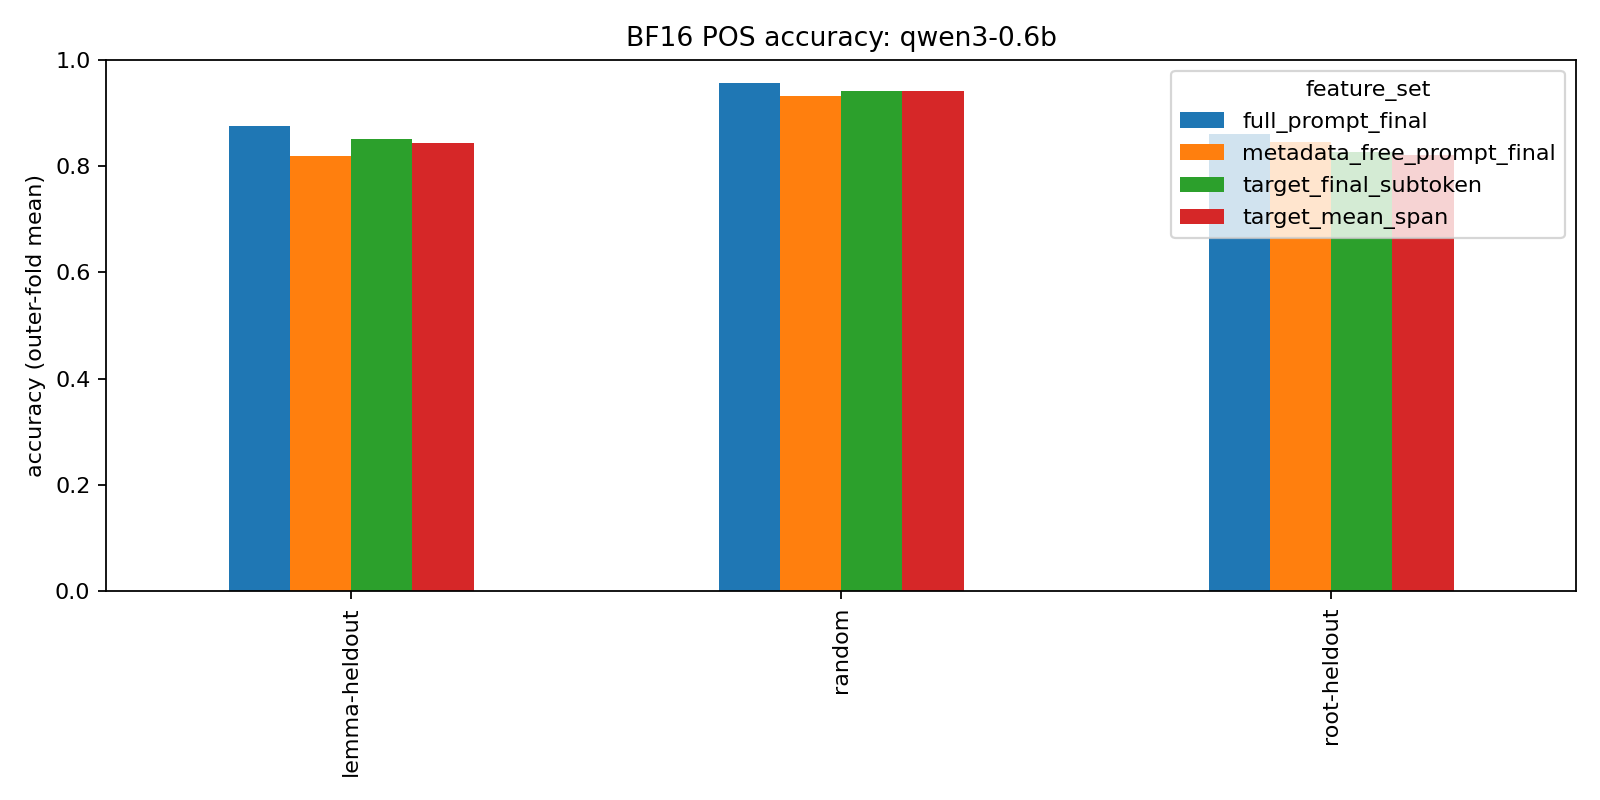
\includegraphics[width=0.96\linewidth]{figures/Fig1_qwen3-0.6b_pos_accuracy.png}
\caption{Generated BF16 POS accuracy summary for Qwen3-0.6B across the three
split conditions and four interfaces. The figure is descriptive; the full
numeric matrix is the CSV artifact}
\label{fig:qwen-pos}
\end{figure}

\begin{figure}[t]
\centering
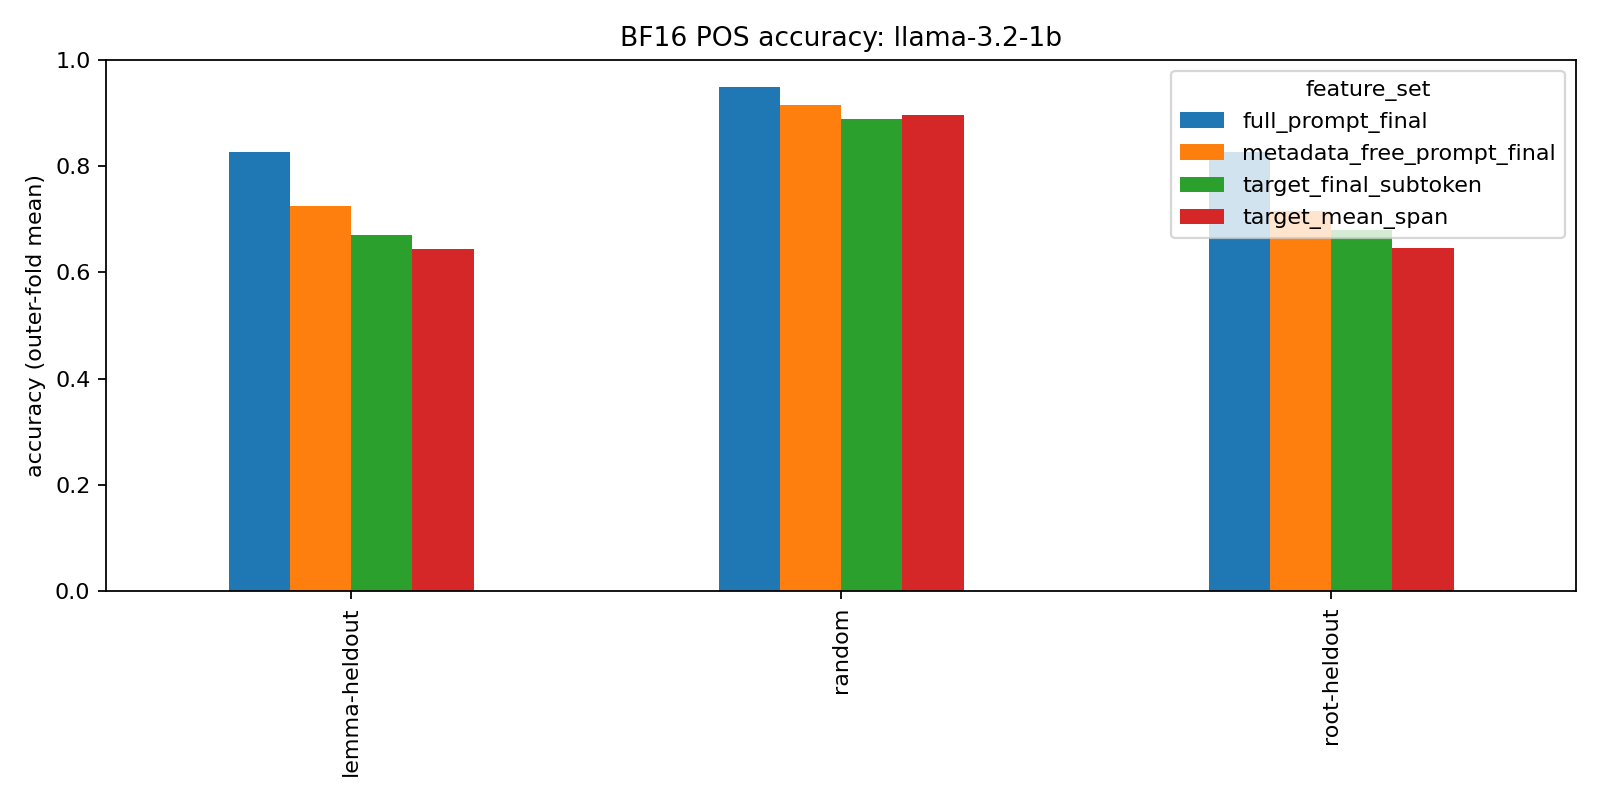
\includegraphics[width=0.96\linewidth]{figures/Fig2_llama-3.2-1b_pos_accuracy.png}
\caption{Generated BF16 POS accuracy summary for Llama-3.2-1B. The paired
figures illustrate model heterogeneity; causal architectural interpretation
requires a controlled design}
\label{fig:llama-pos}
\end{figure}

\subsection{Heterogeneity across models and tasks}

The interface/task summaries in Table~\ref{tab:axis-deltas} show that the
largest descriptive gaps occur for POS when averaged over the matrix (+0.1339
lemma and +0.1498 root). Gender has smaller mean gaps (+0.0854 and +0.1009),
and number is intermediate (+0.0982 and +0.1030). These descriptive values
reflect this dataset, these prompts, these interfaces, and the fixed linear
probe; they describe this matrix, with POS interpretation conditioned on the
same evaluation choices.

Llama-3.2-1B is an informative high-sensitivity case. With target-mean-span
pooling, its number gap is +0.2863 for random minus lemma-heldout and +0.2687
for random minus root-heldout; its POS gaps under the same pooling are +0.2785
and +0.2796. At the other end, the Mistral-7B full-metadata gender row has the
minimum lemma gap in the generated table, +0.0127. These examples characterize
heterogeneity: the amount of apparent random-split advantage depends
materially on the model and task. The matrix supplies no controlled test of
scaling or causal mechanisms.

\begin{table}[t]
\centering
\caption{Descriptive mean macro-F1 gaps by interface and task. Interface rows
average over models and tasks; task rows average over models and interfaces.
All values are computed from the generated split-delta CSV.}
\label{tab:axis-deltas}
\small
\begin{tabular}{lrr}
\toprule
Grouping & Random--lemma & Random--root \\
\midrule
Full-metadata prompt-final & +0.0734 & +0.0948 \\
Metadata-free prompt-final & +0.1138 & +0.1251 \\
Target-final subtoken & +0.1141 & +0.1179 \\
Target mean span & +0.1222 & +0.1337 \\
\midrule
POS & +0.1339 & +0.1498 \\
Gender & +0.0854 & +0.1009 \\
Number & +0.0982 & +0.1030 \\
\bottomrule
\end{tabular}
\end{table}

\subsection{Prompt metadata ablation}

The full-metadata prompt-final state combines representation position with
prompt information. In the Qwen3-0.6B lemma-heldout POS condition, full-metadata
prompt-final macro-F1 is 0.8565, while metadata-free prompt-final macro-F1 is
0.7855. The corresponding target-final-subtoken and target-mean-span values
are 0.8213 and 0.8116. This pattern is consistent with explicit metadata
contributing to the information available at the contextual endpoint. The
aggregate comparison leaves the responsible field or mechanism unresolved.

The ablation yields interface-specific effects. In the
Jais-13B lemma-heldout number condition, metadata-free prompt-final macro-F1
is 0.8272 and full-metadata prompt-final macro-F1 is 0.7249. Similar reversals
occur elsewhere in the full matrix. Prompt-final interface comparisons must
therefore be reported as information-availability comparisons as well as
position comparisons. Importantly, metadata-free prompt-final and target
interfaces remain above their shuffled controls in many settings, so the
explicit-field ablation leaves substantial recoverable signal.

\subsection{Target pooling and representation interface}

Final-subtoken and mean-span pooling change absolute macro-F1 in some cells,
but the larger split-dependent conclusion remains: all 132 interface-specific
random-minus-grouped deltas are positive. Averaged over the matrix,
target-final-subtoken has lemma/root gaps of +0.1141/+0.1179, while
target-mean-span has +0.1222/+0.1337. The mean-span interface therefore shows
somewhat larger descriptive split gaps in this matrix. Pooling order and
linguistic interpretation remain conditional on this matrix and interface.

The complete-span capture is the important methodological safeguard. Because
the raw states for every target-overlapping token are preserved, final-token
and mean-span results are local transformations of the same evidence. A
future pooling analysis within the recorded span is available from the
existing forward pass. Capturing only a final subtoken would have precluded
this robustness question.

\subsection{Controls and class-sensitive interpretation}

The 360 shuffled cells remain at or below their corresponding train-only
majority accuracies. This is a necessary pipeline sanity result; causal use of
the real-label results by the models requires separate evidence. Majority accuracy
is particularly important for number. Across the matrix, the majority
accuracy for number is approximately 0.8415 in the recorded summaries, while
gender and POS majority accuracies are approximately 0.6261 and 0.6290.
The number accuracy values can therefore look strong while macro-F1 remains
limited for minority classes. All main interpretations use both metrics.

The per-class/POS artifact preserves the details needed to check this claim
from archived evidence alone. It reports precision, recall, F1, support, and
confusion matrices for each class, split, interface, and outer fold, together
with gold-POS strata. The fragmentation artifact similarly reports accuracy
and macro-F1 in the 1, 2, and 3+ target-token bins. These analyses are
diagnostic descriptions of where errors occur, separate from the primary
estimands.

\subsection{BF16 relative to historical Q8}

The historical Q8 captures provide robustness and historical context; BF16 is
the primary experiment. For overlapping model/interface/task/split
comparisons, BF16 and historical Q8 agree in majority-relative metric
direction for 105 of 108 fold-zero comparisons. This supports the conclusion
that the broad qualitative contrast between real-label results and the
majority reference extends across two numeric formats.

The comparison measures metric-direction agreement; numerical equivalence
between BF16 and Q8 hidden states would require paired hidden-state arrays.
The raw historical
Q8 feature arrays listed in the v3 external artifact record are absent from the
live checkout, so direct BF16--Q8 vector cosine and relative-L2 comparisons
remain unavailable. The historical Q8 run was neither repeated nor relabeled,
and no vector claim is inferred from the metric-direction result.

\subsection{Supporting CKA/RSA diagnostics}

Fixed-sample CKA and RSA matrices are retained for the two primary models and
are computed only as diagnostics. They document interface similarity while
the task-level probe comparisons measure label recoverability; the two
diagnostic families answer different questions. Since the split, ablation, and
pooling results already answer the planned methodological questions, CKA/RSA
remains a supporting result.

\section{Discussion}

\subsection{What random and grouped splits measure}

Random instance splitting measures performance when the probe may interpolate
among instances drawn from the same lexical inventory as training. This can be
a useful operational condition when deployment also contains repeated lexical
identities; its optimism is a property of the estimand, and it remains a valid
condition. Lemma-
heldout evaluation measures transfer across lemma groups, and
root-heldout evaluation measures transfer across root groups. The consistent
positive gaps in this study show that these estimands differ in the Arabic
resource. The appropriate condition depends on whether the claim concerns
instance-level interpolation or transfer across lexical groups.

The varying size of the gaps matters alongside their direction. The
heterogeneous gaps call for model-, task-, interface-, and grouping-specific
reporting; a single penalty would overcorrect some combinations and undercorrect
others. The compact table serves as an audit summary; any correction must remain
specific to the model, task, interface, and grouping key. Researchers should report the random
reference and the grouping key together,
and should state whether the scientific claim concerns seen-lexicon
interpolation or transfer across the grouping identity.

\subsection{Why split sensitivity varies}

Several mechanisms can produce the observed heterogeneity while leaving
internal model strategy unresolved. Labels may be more lexically predictable
for one task than another; a model may represent orthographic or contextual
cues differently; tokenizers may expose different target fragments; and a
prompt endpoint may integrate fields that are unavailable at the target. The
matrix also confounds architecture, pretraining data, instruction tuning,
parameter count, and tokenizer. The observed ordering therefore reflects a
mixture of these factors, with causal attribution remaining underdetermined.

The matrix offers no clean size trend. The Qwen and Llama subsets provide
within-family size comparisons, while the full design mixes architecture,
training, instruction status, and tokenizer. The model-level table shows
heterogeneity; claims about size-dependent lexical robustness require a more
controlled design.

\subsection{Representation-interface validity}

The prompt metadata ablation clarifies a common ambiguity. A full-metadata
prompt-final state may be highly predictive because the endpoint has access to
fields that summarize lexical and morphological structure. That is a valid
measurement if the question concerns the model's response to the complete
prompt, while a target word state's recoverability requires its own comparison.
The metadata-free condition narrows the information difference, while the
target-prefix condition removes later fields. Both remain contextual and
tokenization-dependent measurements.

Pooling is similarly part of the construct. The final target subtoken gives a
specific causal position but may privilege the last fragment. Mean-span
pooling uses all target-overlapping states and can change both signal and
error patterns. Because substantive split conclusions survive both rules in
the generated table, the lexical-split result survives the historical
final-subtoken choice. That robustness is conditional on the captured span;
generalization to other pooling schemes requires measurement.

\subsection{Scope of Probe-Based Evidence}

Probe performance characterizes information accessible to the estimator at the
chosen representation under a named prompt, split, layer-selection rule, and
estimator. The relationship between that accessibility and the model's causal
generation mechanism remains outside the scope of this study. Lexical
memorization, lexical generalization, linear recoverability, and linguistic
competence describe different properties. Causal interventions, nonlinear
estimators, and behavioral tests would answer different questions and belong
to separate studies.

\subsection{Methodological implications}

For decoder-only morphology probing, the minimum reportable unit should
include the lexical grouping rule, the prompt information available at the
extraction site, the target-to-token alignment, the pooling operation, the
metric and majority reference, and the boundary between development and test
decisions. The present resource makes those decisions auditable and stores the
representation evidence once. This permits later probes, split
reconstructions, error analyses, and representation comparisons to run locally
from archived evidence, eliminating repeated model inference and dependence on
the survival of a cloud instance.

\section{Limitations}

First, the testbed is one resource: Modern Standard Arabic newswire derived
from Arabic-PADT. The findings concern this resource; behavior for other
Arabic genres, dialects, languages, or annotation traditions requires separate
evaluation. The recovered source content
matches official UD r2.17 and r2.18 training files, while the historical local
release label remains unresolved because the original copy retained no Git
metadata. The frozen dataset bytes and exact rebuild remain intact; the
provenance ambiguity should remain visible.

Second, the tasks are POS, gender, and number. Arabic morphology includes
additional features and interactions. The analyzer-derived lemma, root, and
pattern fields are retained for grouping and metadata, while high-cardinality
heldout-label classification falls outside the primary claim. Root and lemma
are linguistically useful grouping variables with limited coverage of lexical
identity.

Third, the primary estimator is linear and fixed. A nonlinear probe, a
different regularization rule, or a different layer-selection policy would
measure a different recoverability profile. The fixed alpha and
development-only layer selection make the current comparisons auditable;
estimator dependence remains.

Fourth, representation interfaces remain contextual and tokenizer-dependent.
Metadata-free prompt-final still includes prompt context, and target states
depend on model-specific subword boundaries. The ablation and pooling checks
reduce known confounds; a unique ``morphology location'' remains unassigned.

Fifth, lexical grouping reduces direct recurrence. Open-set competence remains
untested because surface similarity, morphological patterns, semantics, source
regularities, and tokenizer fragments can cross heldout groups. Conversely,
the model matrix mixes base and instruction-tuned models, so cross-model
causal interpretation of these differences remains underdetermined.

Sixth, uncertainty summaries are conditional. The five-fold standard
deviations summarize the recorded outer folds; the preserved prompt-cluster
bootstrap targets conditional finite-test-set variation under fixed probes,
partitions, and representations. Population or training-seed uncertainty and
causal interventions require separate designs.

Finally, the direct BF16--Q8 vector comparison remains unavailable because
historical Q8 feature arrays are absent from the live checkout. We report only
the verified 105/108 majority-relative direction agreement. This limitation
belongs to the historical artifact record; the Q8 experiment remains the
historical execution with its original labels.

\section{Resource, Code, and Reproducibility Availability}

The complete working package is organized around immutable evidence and
weight-free analysis. It contains:

\begin{itemize}
    \item the frozen normalized stimuli, source release record, transformation
    code, field lineage, and dataset hashes;
    \item prompt templates, per-example rendered prompts and hashes, exact
    target character and byte spans, token IDs and pieces, and alignment
    records;
    \item the pinned eleven-model manifest with repository, revision, config,
    tokenizer revision, architecture, dtype contract, licensing/access
    status, expected dimensions, and resource estimates;
    \item validated BF16 hidden-state bundles containing all layer-wise
    prompt-final states and all target-span token states, together with
    manifests, commands, runtime metadata, checksums, and completion records;
    \item deterministic split manifests, five-fold result cells, primary-model
    predictions, majority and shuffled controls, fragmentation and class/POS
    error analyses, BF16/Q8 comparison records, and fixed CKA/RSA diagnostics;
    \item the local loaders and analysis runner, a sufficiency audit showing
    that planned post-extraction analyses can use archived representations
    alone, and a content-addressed BF16 analysis freeze.
\end{itemize}

The primary analysis source is \bfana. Its complete dataset and model-matrix
hashes are recorded in the run manifest, frozen snapshot, and quantitative
claim ledger. The freeze verifier passed for
\texttt{evidence/bf16-analysis-20260826-v2/}. The
historical LRE v3 freeze and historical Q8 run remain separate, immutable
records; this manuscript leaves them unchanged.

Reproduction begins by verifying the dataset, model-matrix, bundle, and
analysis-freeze hashes, then running the local analysis command against the
frozen run root. Model weights are needed only for a new extraction. The
current planned analysis state has \texttt{weights\_required=false}; the saved
captures are the scientific representation evidence.

\section{Conclusion}

This study evaluates lexical split design and representation-interface design
as part of the measurement construct in decoder-only morphology probing. In
the completed BF16 Arabic matrix, random instance splits produce higher
macro-F1 than both lemma-heldout and root-heldout evaluation in every
model--task--interface row, but the size of that advantage varies materially.
The result supports a condition-specific interpretation of split gaps: split
choice changes the question being answered.

The same qualification applies to representation position. A full-metadata
prompt-final state can access explicit lemma, root, and pattern fields, while
target and metadata-free interfaces make different information available and
use different contextual boundaries. Final-subtoken and mean-span pooling
provide locally recoverable alternatives when the complete target span is
archived. Robust morphology probing should report these choices together and
interpret scores as linear recoverability under the stated interface. Causal
model use and unrestricted linguistic competence require separate evidence.

\appendix

\section{Exact model identities and access metadata}\label{app:models}

Table~\ref{tab:model-matrix} records the full model identity used by the BF16
run. The exact manifest additionally records expected BF16 weight size, VRAM
estimate, context length, minimum and recommended AWS instance, gated status,
access status, and trust-remote-code policy. The model list serves robustness
across selected families, with scaling effects outside its design.

\scriptsize
\setlength{\tabcolsep}{2pt}
\begin{longtable}{@{}>{\raggedright\arraybackslash}p{1.45cm}
>{\raggedright\arraybackslash}p{2.25cm}
>{\raggedright\arraybackslash}p{4.35cm}
>{\raggedright\arraybackslash}p{2.35cm}@{}}
\caption{Pinned BF16 model matrix. Repository revisions are full commit SHAs;
tokenizer and config revisions equal the listed model revision for every row.
The manifest is authoritative for licenses, gated status, access status, and
all resource estimates.}\label{tab:model-matrix}\\
\toprule
Model & Architecture and size & HF repository and pinned revision & Dtype; hidden; role \\
\midrule
\endfirsthead
\toprule
Model & Architecture and size & HF repository and pinned revision & Dtype; hidden; role \\
\midrule
\endhead
\bottomrule
\endfoot
\texttt{qwen3-}\newline\texttt{0.6b} & \texttt{Qwen3For}\newline\texttt{CausalLM}; 0.6B & \texttt{Qwen/Qwen3-0.6B}\newline
\texttt{c1899de289}\newline\texttt{a04d12100d}\newline\texttt{b370d81485}\newline\texttt{cdf75e47ca} & bf16 / bf16; 1024 / 28;\newline Qwen size-small \\
\texttt{qwen2.5-}\newline\texttt{1.5b} & \texttt{Qwen2For}\newline\texttt{CausalLM}; 1.5B & \texttt{Qwen/Qwen2.5-1.5B-}\newline\texttt{Instruct}\newline
\texttt{989aa7980e}\newline\texttt{4cf806f80c}\newline\texttt{7fef2b1adb}\newline\texttt{7bc71aa306} & bf16 / bf16; 1536 / 28;\newline Qwen size-medium \\
\texttt{qwen3-8b} & \texttt{Qwen3For}\newline\texttt{CausalLM}; 8B & \texttt{Qwen/Qwen3-8B}\newline
\texttt{b968826d9c}\newline\texttt{46dd6066d1}\newline\texttt{09eabc6255}\newline\texttt{188de91218} & bf16 / bf16; 4096 / 36;\newline Qwen size-large \\
\texttt{llama-}\newline\texttt{3.2-1b} & \texttt{LlamaFor}\newline\texttt{CausalLM}; 1B & \texttt{meta-llama/}\newline\texttt{Llama-3.2-1B-Instruct}\newline
\texttt{9213176726}\newline\texttt{f574b55679}\newline\texttt{0deb65791e}\newline\texttt{0c5aa438b6} & bf16 / bf16; 2048 / 16;\newline Llama size-small \\
\texttt{llama-}\newline\texttt{3.2-3b} & \texttt{LlamaFor}\newline\texttt{CausalLM}; 3B & \texttt{meta-llama/}\newline\texttt{Llama-3.2-3B-Instruct}\newline
\texttt{0cb88a4f76}\newline\texttt{4b7a12671c}\newline\texttt{53f0838cd8}\newline\texttt{31a0843b95} & bf16 / bf16; 3072 / 28;\newline Llama size-medium \\
\texttt{llama-}\newline\texttt{3.1-8b} & \texttt{LlamaFor}\newline\texttt{CausalLM}; 8B & \texttt{meta-llama/}\newline\texttt{Meta-Llama-3.1-8B-Instruct}\newline
\texttt{0e9e39f249}\newline\texttt{a16976918f}\newline\texttt{6564b8830b}\newline\texttt{c894c89659} & bf16 / bf16; 4096 / 32;\newline Llama size-large \\
\texttt{gemma-}\newline\texttt{4-2b} & \texttt{Gemma4For}\newline\texttt{Conditional}\newline\texttt{Generation}; E2B & \texttt{google/gemma-4-E2B-it}\newline
\texttt{3e22461f65}\newline\texttt{e89153144f}\newline\texttt{8adb70e3b8}\newline\texttt{c2cc9845a7} & bf16 / bf16; 1536 / 35;\newline Cross-family \\
\texttt{phi-3-}\newline\texttt{mini} & \texttt{Phi3For}\newline\texttt{CausalLM}; 3.8B & \texttt{microsoft/}\newline\texttt{Phi-3-mini-4k-instruct}\newline
\texttt{f39ac1d28e}\newline\texttt{925b323eae}\newline\texttt{81227eaba4}\newline\texttt{464caced4e} & bf16 / bf16; 3072 / 32;\newline Cross-family \\
\texttt{mistral-}\newline\texttt{7b} & \texttt{MistralFor}\newline\texttt{CausalLM}; 7B & \texttt{mistralai/}\newline\texttt{Mistral-7B-Instruct-v0.3}\newline
\texttt{c170c708c4}\newline\texttt{1dac9275d1}\newline\texttt{5a8fff4eca}\newline\texttt{08d52bab71} & bf16 / bf16; 4096 / 32;\newline Cross-family \\
\texttt{jais-13b} & \texttt{JAISLMHead}\newline\texttt{Model}; 13B & \texttt{inceptionai/Jais-13B}\newline
\texttt{0d5eb87f91}\newline\texttt{e6577dac17}\newline\texttt{bc319eee94}\newline\texttt{0fb875b899} & fp32 / bf16; 5120 / 40;\newline Arabic-specialist \\
\texttt{allam-7b} & \texttt{LlamaFor}\newline\texttt{CausalLM}; 7B & \texttt{ALLaM-AI/}\newline\texttt{ALLaM-7B-Instruct-preview}\newline
\texttt{a28dd1e674}\newline\texttt{20cde72d36}\newline\texttt{29c8633a97}\newline\texttt{4cf7d9c366} & bf16 / bf16; 4096 / 32;\newline Arabic-specialist \\
\end{longtable}
\normalsize

The manifest's access metadata records Qwen3-0.6B, Qwen2.5-1.5B, Qwen3-8B,
Gemma-4-E2B-it, Phi-3-mini, Mistral-7B-Instruct-v0.3, and ALLaM-7B as
non-gated public entries; the Qwen entries use Apache-2.0, Gemma uses its
terms of use, Phi uses MIT, Mistral uses Apache-2.0, and ALLaM's model license
is recorded as a model-specific license requiring card verification. Llama
3.2-1B, Llama 3.2-3B, Llama 3.1-8B, and Jais-13B are gated entries with the
respective Llama community or Jais access requirements in the manifest. Only
Jais has \texttt{trust\_remote\_code=true}; all other rows use the manifest's
false value. The tokenizer and config revisions equal the model revision in
every row. These fields record model access and licensing directly in the
frozen identity manifest.

\section{Representation bundle schema}\label{app:bundle-schema}

For each model and prompt condition, the self-contained bundle has the
following logical structure:

\begin{verbatim}
manifest.json
model.json / tokenizer.json / prompt.json
examples.jsonl
alignment.jsonl
representations/
  embedding_output.safetensors
  layer_0000.safetensors ... layer_<last>.safetensors
validation.json
checksums.sha256
COMPLETE
\end{verbatim}

Each layer file contains a prompt-final matrix with shape
$[N,H]$ and a flattened target-span matrix with shape $[\sum_i T_i,H]$,
where $N$ is the number of examples, $H$ is hidden size, and $T_i$ is the
validated target token count for example $i$. The embedding file contains the
embedding-output matrix with shape $[N,H]$. The complete target span makes
final-subtoken and mean-span pooling local operations. Tensor validation
rejects missing layers, shape mismatches, duplicate IDs, NaNs, and infinities.

\section{Complete result and audit artifacts}\label{app:artifacts}

The complete model-by-task-by-interface split table is generated at
\texttt{evidence/bf16-analysis-20260826-v2/snapshot/analysis/results/}
\texttt{/macro\_f1\_split\_deltas.csv}, with synchronized Markdown and TeX
renderings. The source \texttt{summary.csv} contains 396 rows, each with five
folds, accuracy, macro-F1, train-only majority accuracy, above-majority gap,
and selected-layer records. The detailed cell JSON files preserve each fold's
development layer metrics, selected layer, test metrics, and control metadata.

The audit package also contains:

\begin{itemize}
    \item \texttt{shuffled\_controls.csv} for the 360 primary-model control
    cells;
    \item \texttt{fragmentation.csv} with target token-count bins 1, 2, and
    3+;
    \item \texttt{class\_pos\_error\_analysis.csv} with per-class and
    POS-stratified errors;
    \item \texttt{bf16\_q8\_comparison.json} with the 105/108
    majority-relative direction record and the unavailable vector-comparison
    status;
    \item \texttt{cka\_rsa\_diagnostics.json} and
    \texttt{analysis\_decision.md}, documenting the supporting-only status of
    CKA/RSA;
    \item \texttt{local\_analysis\_sufficiency.json}, which records the
    fields consumed by the planned analysis and
    \texttt{weights\_required\_after\_capture=false}.
\end{itemize}

\section{Quantitative claim and provenance ledger}\label{app:ledger}

The manuscript's claim-to-artifact mapping is supplied alongside this source
as \texttt{quantitative\_claim\_map.md}. It maps every numerical claim to the
generated result, dataset provenance, model manifest, or audit record that
produces it. The manuscript reports numerical results only when a generating
artifact is available; direct Q8 vector comparisons and ungenerated analyses
therefore remain unquantified.

\backmatter

\bmhead{Acknowledgements}
During preparation of this manuscript, the author used generative AI tools,
including OpenAI Codex and DeepSeek-based tools, for limited editorial
assistance and software/documentation support. The author reviewed and
verified the manuscript, citations, code, data, analyses, and reported claims
and retains full responsibility for the final work.

\bmhead{Statements and Declarations}

\bmhead{Funding}
This study received no external funding. The work was self-funded by the
author.

\bmhead{Competing interests}
The author declares no competing financial or non-financial interests related
to this work.

\bmhead{Ethics approval and consent to participate}
Ethics approval was not required because this study analyzes a public,
pre-existing annotated linguistic resource and involved no recruitment or
interaction with human participants.

\bmhead{Consent for publication}
Not applicable. The study uses a public, pre-existing linguistic resource and
reports aggregate analysis results; no individual participant data are
presented.

\bmhead{Data availability}
The compact code, provenance, analysis, and validation package is publicly
available in the source archive at
\url{https://github.com/voidwest/arabic-morphology-probing-lre}. The repository
contains the reproducibility manifests, generated results, validation reports,
and checksums. The raw representation bundles, including those derived from
Meta Llama, Jais, and ALLaM checkpoints, are not publicly redistributed. Any
separate request is considered only after the requester independently obtains
the corresponding checkpoint authorization, accepts the applicable model-card
and license terms, and the transfer is permitted under those terms. No model
weights, credentials, or Hugging Face tokens are shared; when these conditions
cannot be confirmed, the raw bundle is not provided.

\bmhead{Materials availability}
The dataset, prompt specifications, split manifests, model manifest, and
derived analysis artifacts are described in the Resource, Code, and
Reproducibility Availability section and in the public source archive at
\url{https://github.com/voidwest/arabic-morphology-probing-lre}. Public
redistribution is limited to the compact artifacts committed there. The
license-aware policy for external raw bundles and card-restricted model
derivatives is documented in \texttt{EXTERNAL\_ARTIFACTS.md}; no raw gated-model
bundle is anonymously downloadable from the archive.

\bmhead{Code availability}
The extraction, validation, split, probe, and reporting code is included in
the public source archive at
\url{https://github.com/voidwest/arabic-morphology-probing-lre}.

\bmhead{Author contribution}
Mohammed Al-Thobaiti: Conceptualization, Methodology, Software, Validation,
Formal analysis, Investigation, Data curation, Writing---original draft,
Writing---review and editing, Visualization, and Project administration.

\bibliography{references}

\end{document}
